%%%%%%%%%%%%%%%%%%%%%%% file template.tex %%%%%%%%%%%%%%%%%%%%%%%%%
%
% This is a template file for Web of Conferences Journal
%
% Copy it to a new file with a new name and use it as the basis
% for your article
%
%%%%%%%%%%%%%%%%%%%%%%%%%% EDP Science %%%%%%%%%%%%%%%%%%%%%%%%%%%%
%
%%%\documentclass[option]{webofc}
%%% "twocolumn" for typesetting an article in two columns format (default one column)
%
\documentclass{webofc}
\usepackage[varg]{txfonts}   % Web of Conferences font
\usepackage{float}
\usepackage{natbib} 
%
% Put here some packages required or/and some personnal commands
%
\usepackage{graphicx}
\begin{document}
%
\title{dCache: from Resilience to Quality of Service}
%
% subtitle is optionnal
%
%%%\subtitle{Do you have a subtitle?\\ If so, write it here}

\author{\firstname{Albert} \lastname{Rossi}\inst{2}\fnsep\thanks{\email{arossi@fnal.gov}} 
        \firstname{Krishnaveni} \lastname{Chitrapu}\inst{3},
        \firstname{Vincent} \lastname{Garonne}\inst{4},
        \firstname{Dmitry} \lastname{Litvintsev}\inst{2},
        \firstname{Svenja} \lastname{Meyer}\inst{1},
        \firstname{Paul} \lastname{Millar}\inst{1},
        \firstname{Tigran} \lastname{Mkrtchyan}\inst{1},
        \firstname{Lea} \lastname{Morschel}\inst{1}, \and
        \firstname{Marina} \lastname{Sahakyan}\inst{1}
}

\institute{Deutches Elektronen-Synchrotron DESY, Hamburg, Germany   
\and
           Fermi National Accelerator Laboratory FNAL, Batavia, USA
\and
           National Super Computer Center, Link\"oping University, Sweden
\and
           Nordic e-Infrastructure Collaboration, University of Oslo, Norway
          }

\abstract{%
  A major goal of future dCache development will be to allow
  users to define file Quality of Service (QoS) in a more flexible way
  than currently available.  This will mean implementing what might be
  called a  QoS rule engine  responsible for registering  and managing
  time-bound  QoS   transitions  for  files  or   storage  units.   In
  anticipation of this extension  to existing dCache capabilities, the
  Resilience service, which maintains  on-disk replica state, needs to
  undergo both structural modification and generalization.  This paper
  describes  ongoing  work  to   transform  Resilience  into  the  new
  architecture which  will eventually  support a more  broadly defined
  file QoS.  }
%
\maketitle
%
\section{Introduction}
\label{intro}

dCache \cite{dcache,Tigran} is an open-source distributed storage system, 
designed and proven to be dynamically scalable to hundreds of petabytes 
in capacity. The system can be configured as a stand-alone disk-only
system or in combination with an arbitrary tape storage system. In the latter 
configuration, dCache plays the role of a distributed disk buffer 
that hides inefficiencies associated with the high latency and sequential 
nature of tape access from the end user. Additionally, dCache can be 
configured as a multi-tier storage solution incorporating storage 
devices of varying throughput capacities with seamless migration 
of the data between the tiers.  

dCache has been used predominantly by the scientific community to
store data for research in a wide variety of disciplines, performed
by groups ranging from a few individuals to international collaborations
of many thousands of members, and with different work-flows, access, 
capacity and data preservation requirements, resources and budgets. 
Therefore, there can be a considerable difference
in the  scientists’ desires  and expectations about  how this  data is
stored and made  available for analysis.  These  expectations could be
in  terms of  durability (likelihood  of data  loss), total  bandwidth
(aggregated over all clients), bandwidth available to a single client,
access latency or some combination of these factors.

Some expectations  may be based  on intrinsic properties of  the data;
for example, raw observational data  may be extremely precious because
it is impossible  to reproduce.  The scientists  may accept additional
storage costs or  increased latency if this reduces  the likelihood of
data loss.  Other  expectations may be based on  current activity; for
example, if a particular set of  files will be read by many concurrent
analysis  jobs, then  storing multiple  copies of  these files  allows
dCache  to  provide  sufficient  aggregate bandwidth  to  satisfy  all
clients.  Similarly, if a small amount  of data is expected to provide
input to an I/O-bound analysis job, then it may be useful for that data
to be stored on specialized, low-latency media.

Exposing all  possible storage options would overwhelm users. 
Thus it is desirable to have specific, fixed data
placement strategies  that provide particular storage  and performance
characteristics.  These  different strategies are called  QoS (Quality
  of Service)  Classes \cite{Millar:2017czb}.  By allowing  scientists to choose  and modify
with which  QoS Class  they would  like their  data stored,  a storage
system gives  scientists the  ability to  achieve the  optimal storage
strategy within the available storage capacity.

\section{The dCache Resilience Service as QoS Service}
\label{sec-1}


"Resilience" [henceforward referred to in capitals without quotation marks] 
is a  dCache subsystem  that achieves  data durability  by
maintaining permanent disk replicas independently of the presence of a
back-end  or tertiary  storage system \cite{Rossi:2017hxn}.  
 As implemented,  Resilience
relies on  a partitioning of storage  in such a way  that files, pools
and pool groups are either “resilient”  or not, with the service only
being responsible for handling the former.

With the  advent of  interest in providing  general quality-of-service
management, it was quickly understood that file resilience comprised a
subset  of the  associated and  more broadly  defined objectives.   In
design discussions  of what  will henceforward be  referred to  as the
“QoS Engine”, the reuse of as  much of Resilience as possible was thus
held to be  desirable; there were, however,  considerable obstacles in
its path.  A significant amount of Resilience’s architecture needed to
be re-factored  in order  to be  able to  place on  top of  the already
implemented  functionality the  new set  of semantics  concerning file
status and QoS requirements.

Although the specification of QoS  in dCache remains an unsettled area
of ongoing  investigation and  deliberation, it has  nevertheless been
agreed that,  in advance of  implementing any new  requirements layer,
what exists in  Resilience must be reworked for  easy adaptation.  The
following discussion  will demonstrate  the changes  we are  making to
Resilience  in order  to transform  it into  a set  of QoS  components
supporting   the  QoS   Engine.   All   of  the   previous  Resilience
functionality  will  be retained  in  this  transformation, and  after
sufficient trial  in a  production environment, the  former Resilience
service will  be deprecated and  replaced by  the new QoS  Engine.  At
present, the prototype  is being reviewed for inclusion  in the dCache
code base.

\begin{figure}[h]
\centering
\includegraphics[width=13cm,clip]{fig-1.png}
\caption{dCache Resilience: inter-component interaction (new file write).}
\label{fig-1} 
\end{figure}


\section{Architectural Changes to Resilience and QoS Component Interactions}
\label{sec-2}


Since the original  purpose of Resilience was  narrowly defined, there
was  no need  for  a  clear separation  into  components.  One of  the
original considerations for keeping much of the functionality together
was, in fact,  a concern over efficiency; in particular,  we wished to
minimize inter-service communication via messaging.  During the course
of use in  production, however, it was discovered  that some revisions
to  the  original  communication  model (particularly a significant increase 
in the  number  of messages sent to the pools) were  necessary in order 
to guarantee that the information from the namespace obtained by Resilience 
was actually consistent with  that on the  pools.  There were subtle  
timing issues which  could under  exceptional conditions  lead to incorrect 
replica caching.  Now that  we have had to enact  more aggressive verification
via   messaging,  the   additional   communication  between   separate
components becomes  less significant,  masked by  the traffic  to each
pool in the pool group during any given file update.
\begin{figure}[h]
\centering
\includegraphics[width=12cm,clip]{fig-2.png}
\caption{Resilience service architecture.}
\label{fig-2} 
\end{figure}
The  implicit component  layers in  Resilience have  thus been  teased
apart.  These are based on the following functions:
\begin{enumerate}
\item  determining the number of replicas required;
\item  verifying how many viable replicas there are in the current state of the system;
\item making the adjustments necessary to meet the requirements;
\item reacting to changes in pool status and periodically checking for consistency.
\end{enumerate}

For the QoS Engine, at least the first of these needs to be independent from the rest of the mechanism that maintains a file’s QoS requirements or which transitions it from one set of requirements to another.  But optimal design would also argue for the loose coupling of all four components.

In our 2017 paper \cite{Rossi:2017hxn}, we presented the architecture of the Resilience service (Figures~\ref{fig-1},\ref{fig-2}).


The left-hand column of the diagram in figure~\ref{fig-2} represents the classes (handlers and map) dedicated to processing incoming updates for replica consistency.  The right-hand column represents the classes (handler and map) responsible for intercepting pool status changes or for periodic scheduling of pool scans.  The middle column represents the data components used by Resilience to determine file and pool state.   

For the QoS Engine, we have split out the implicit resilience functions into these explicit components and interfaces (the first function named above has been further subdivided, for reasons we will make clear below):


\begin{enumerate}

\item  {\bf Receiver:}  receives messages concerning new files and file status changes;
\item  {\bf Provider:}  queried by file and returns the file’s requirements;
\item  {\bf Verifier:}  checks the current status of a file and recommends action, if any;
\item  {\bf Adjuster:}  receives an actionable request for a single operation/transformation (stage, flush, copy, cache);
\item  {\bf Scanner:}  receives messages concerning pool status changes, and schedules periodic scanning of pools.

\end{enumerate}



It is important to note that the responsibilities of each component now have to do with the entire dCache namespace, not just with files that have been marked as resilient by their storage requirements and actual location within designated pool groups.  Note also that Resilience did not trigger the migration of a file to an HSM-backed pool for flushing, because it was not intended to handle the dynamic transitioning of a file from one QoS definition to another.

Figure~\ref{fig-3} gives an overview of how the basic Resilience components have been remapped into these QoS roles.

\begin{figure}[h]
\centering
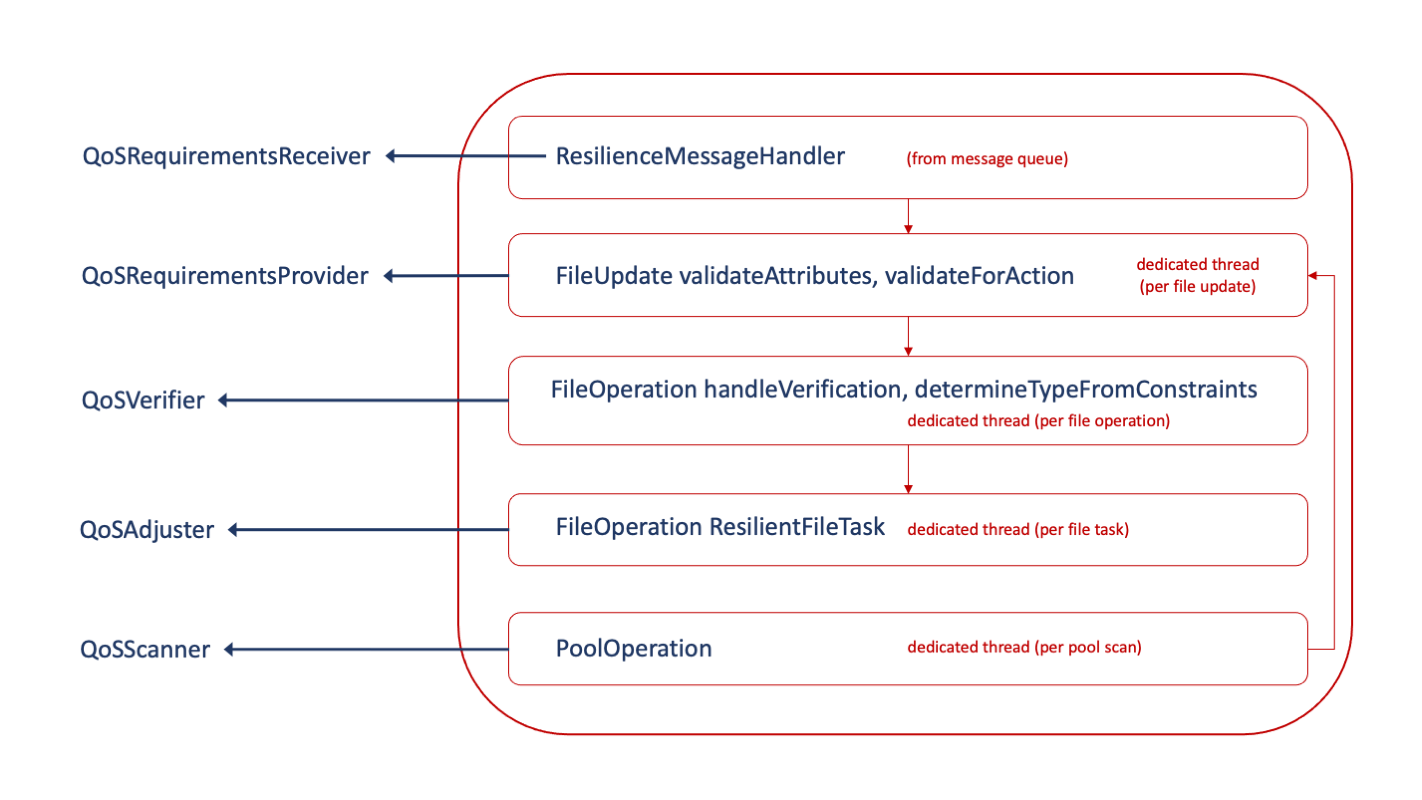
\includegraphics[width=13cm,clip]{fig-3.png}
\caption{Resilience-to-QoS Mapping.}
\label{fig-3} 
\end{figure}

As may be apparent from this diagram, only the message receiver and the pool scanning operations directly converted to the new components; otherwise, some effort was required to split apart internally the left and center stacks on the original diagram.  In particular, the FileOperationHandler and FileOperationMap originally managed both replica verification and adjustment; in addition, elements of the handler conducted a triage on the basis of file requirements it also fetched from the embedded data map and the namespace.  

Figure~\ref{fig-4} illustrates the interactions between the newly defined layers.

\begin{figure}[h]
\centering
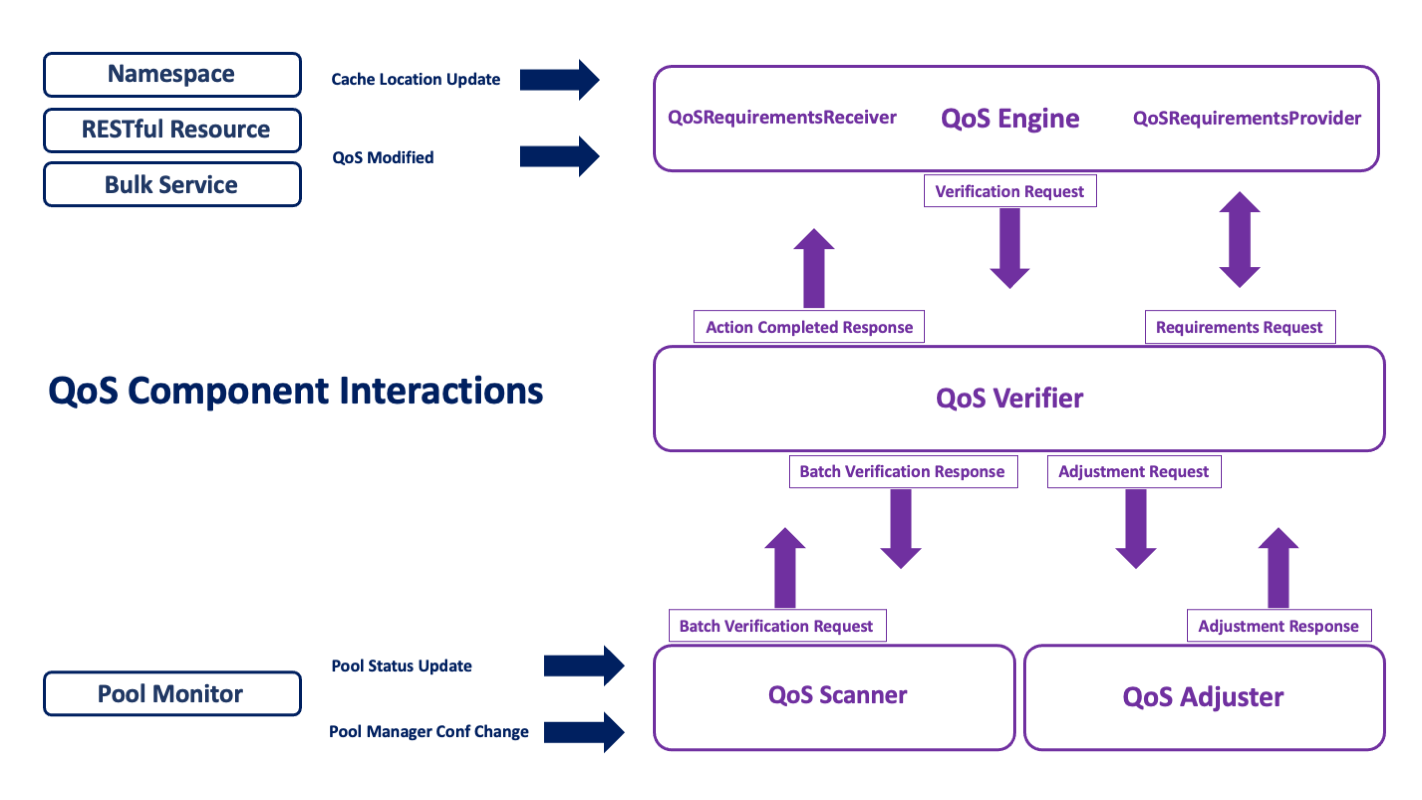
\includegraphics[width=13cm]{fig-4.png}
\caption{QoS Component Interactions.}
\label{fig-4} 
\end{figure}

We have grouped the first two components into what we are calling the “QoS Engine” because it serves as the head or entry point service.  Each of the four components can be run as separate dCache services, with the usual flexibility as to their distribution in domains and over nodes.  We have also provided a standalone version of the entire stack where all components are plugged into each other in the same JVM, avoiding message passing.  This can be used on systems where horizontal scaling is less important but hardware resources are limited (the standalone service requires more memory, of course).

Just as the heart of Resilience lay in the components which queued the file operations and determined how much additional work was necessary to fulfill their replica requirements, the core controlling component in the QoS Engine is the verifier, to which all the other components report.   It is the verifier which decides when a QoS request has completed or failed; it passes off work to the adjuster one action at a time.  This re-factoring also afforded us the opportunity to revise the verifier’s state machine in order to allow for greater compatibility with manual migration during pool draining (which was somewhat problematic in Resilience).

The time-line diagram in figure~\ref{fig-5} illustrates the processing of new files or modification requests:
\begin{figure}[h]
\centering
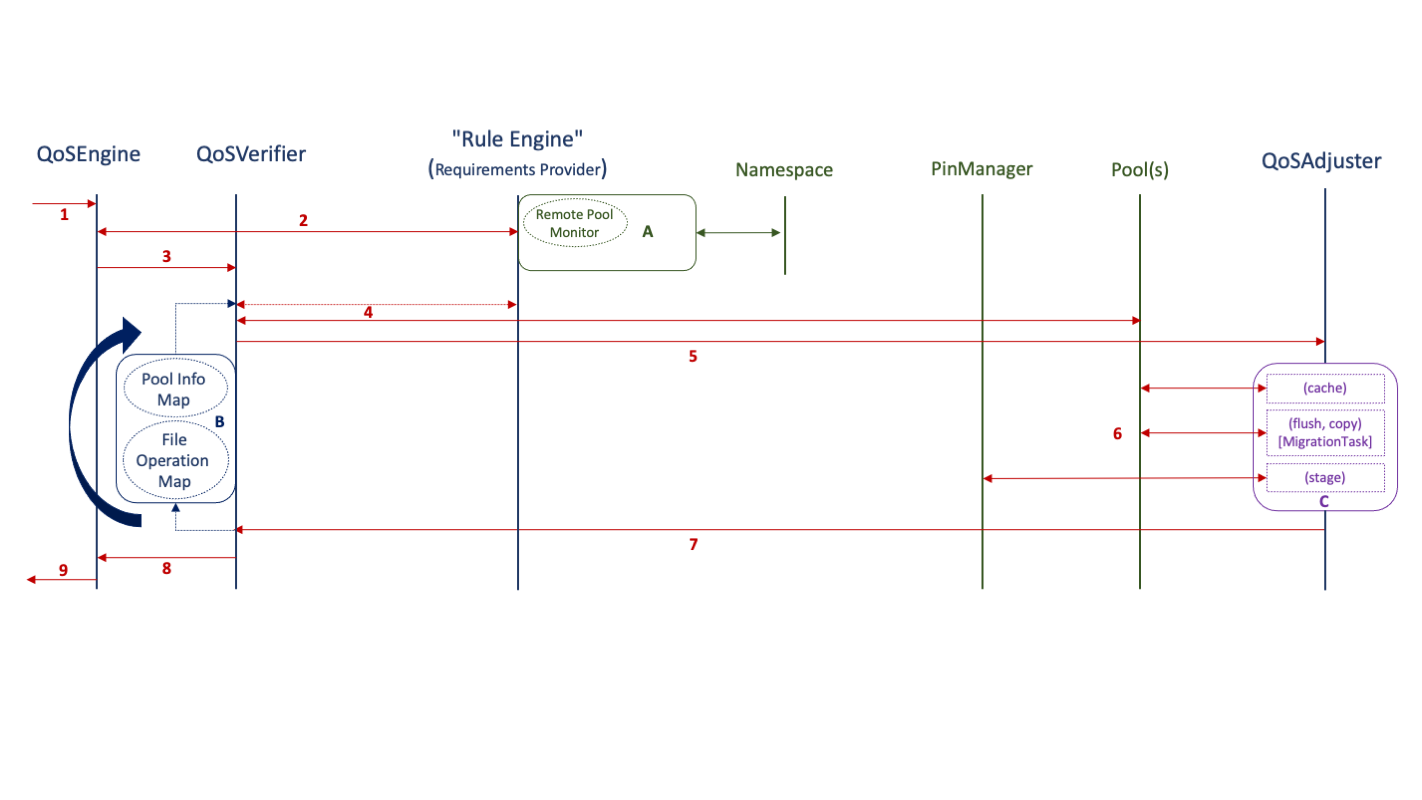
\includegraphics[width=14cm,clip]{fig-5.png}
\caption{QoS Request Handling. A - the current rule engine uses the namespace and Pool Selection Unit. B - The pool selection is done by the verifier and sent as part of the message to the adjuster; verifier keeps track of maximum running slots and only sends ready tasks to the adjuster.
C - The adjuster queues the requests, maps them to adjuster types and executes; the types call out to either the pools or the PinManager.}
\label{fig-5} 
\end{figure}
\begin{figure}[h]
\centering
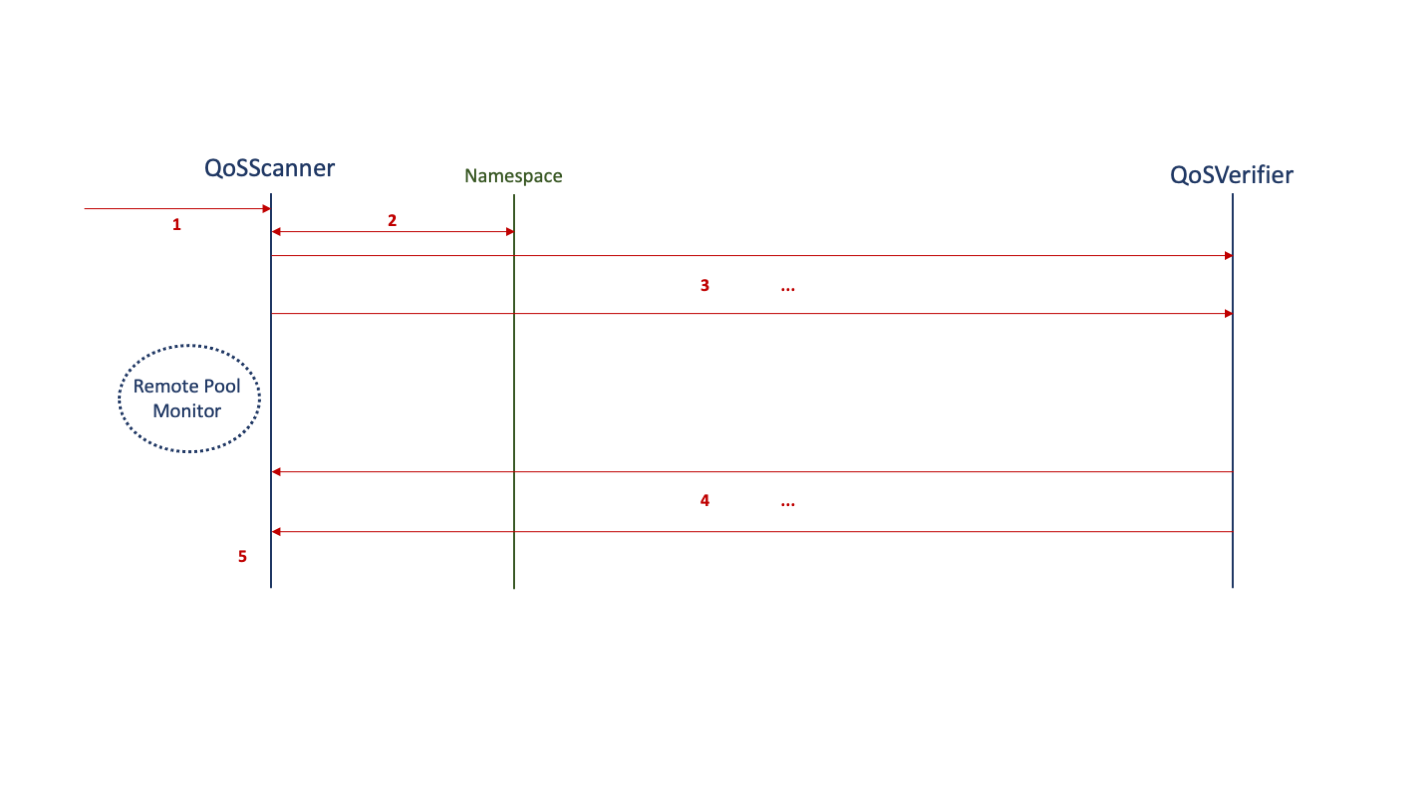
\includegraphics[width=14cm,clip]{fig-6.png}
\caption{QoS Pool/Location Scanning. }
\label{fig-6} 
\end{figure}
\begin{enumerate}
\item receive message (cache update or QoS modification);
\item check the file requirements;
\item request verification;
\item verify the status of the file (how many replicas, on tape, etc.) on the pools (and recontact provider on iteration);
\item determine action, and request adjustment;
\item process the task; if it fails, possibly retry;
\item notify verifier of success/failure; verifier reevaluates for further action (retry, continue to new action, quit);
\item remove operation and send verification/action completed message;
\item notify QoS transition completed (topic).
\end{enumerate}
Figure~\ref{fig-6} shows the location/pool scanning call sequence:
\begin{enumerate}
\item receive message and queue corresponding pool operation;
\item query namespace for files on pool;
\item batching the files, send request to verifier;
\item listen on operation completed topic for the number of files processed;
\item put operation on idle queue when last file is processed.
\end{enumerate}
\begin{table}[H]
\scriptsize
\centering
\caption{Prototype Mapping of dCache Attributes to QoS Classes.}
\label{tab-1}       % Give a unique label
% For LaTeX tables you can use
\begin{tabular}{llllll}
\hline
ACCESS  & RETENTION  &  storage unit & storage unit  & QoS & Description  \\
LATENCY & POLICY  &  -required &  -onlyOneCopyPer &  Class &   \\\hline
NEARLINE & REPLICA & N/A & N/A & {\bf volatile} & could be removed at any time \\
NEARLINE & CUSTODIAL &  N/A & N/A &  {\bf tape } & on tape; disk copy \\
         &           &      &     &              & could be removed at any time \\
ONLINE &  REPLICA & undefined, 1 &  N/A &  {\bf disk } & persistent on disk but not written to tape \\ 
ONLINE & REPLICA & $k > 1$ & partitioned by tags & {\bf disk }& k replicas persistent on disk\\
       &         &        &                      &            &  but not written to tape \\
ONLINE &  CUSTODIAL &  undefined, 1 & N/A &  {\bf disk+tape } &  persistent on disk and one copy on tape \\ 
ONLINE & CUSTODIAL & $k > 1$ & partitioned by tags & {\bf disk+tape} & k replicas persistent on disk\\
       &           &        &                     &                 &  and one copy on tape\\\hline
\end{tabular}
% Or use
\vspace*{5cm}  % with the correct table height
\end{table}
\begin{table}[H]
\scriptsize
\centering
\caption{Prototype QoS Transitions and How They Are Implemented.}
\label{tab-2}       % Give a unique label
% For LaTeX tables you can use
\begin{tabular}{lll}
\hline
 \multicolumn{1}{c}{QoS transition} &  \multicolumn{1}{c}{Change in namespace} &  \multicolumn{1}{c}{Effect} \\\hline
{\bf volatile => disk} &  NEARLINE REPLICA => ONLINE REPLICA &  k replicas are copied or made “sticky” \\
{\bf volatile => tape} & NEARLINE REPLICA => NEARLINE CUSTODIAL & file is migrated to tape-backed pool, if necessary,\\
                       &                                       &  and then flushed \\
{\bf volatile => disk+tape} &  NEARLINE REPLICA => ONLINE CUSTODIAL &  file is migrated to tape-backed pool flushed; \\
                          &                                       & k replicas are copied or made “sticky” \\
{\bf disk => tape } &  ONLINE REPLICA => NEARLINE CUSTODIAL &  file is migrated to tape-backed pool and flushed; \\
                   &                                        &         all replicas are cached \\ 
{\bf disk => disk+tape } & ONLINE REPLICA => ONLINE CUSTODIAL & file is migrated to tape-backed pool and flushed \\
{\bf tape => disk} & NEARLINE CUSTODIAL => ONLINE REPLICA & NOT SUPPORTED \\ 
{\bf tape => disk+tape} & NEARLINE CUSTODIAL => ONLINE CUSTODIAL& k replicas made ``sticky'' or copied \\ 
{\bf tape => disk+tape } &  NEARLINE CUSTODIAL => ONLINE CUSTODIAL &  file not currently on disk;\\
                         &                                        &  file is staged from tape; k replicas are copied \\ 
{\bf disk+tape => tape} &  ONLINE CUSTODIAL => NEARLINE CUSTODIAL &  all replicas are cached \\
{\bf disk+tape => disk}  & ONLINE CUSTODIAL => ONLINE REPLICA & NOT SUPPORTED \\\hline
\end{tabular}
% Or use
\vspace*{5cm}  % with the correct table height
\end{table}


A crucial aspect of the separation into components is that it permits an easier redefinition of the QoS Engine “peripherals”–– that is, the adjuster and provider layers. 
 

\subsection{QoS Adjuster}

This service encapsulates a number of tasks which either call out to the pools directly to change the replica’s meta-data (such as the “sticky” bit designating its permanence on disk), to copy it or migrate it for flushing, or to request staging through the PinManager.   The tasks are rather simple and rely on other parts of dCache to do most of the work.  Nevertheless, they do contain some logic (such as synchronous waiting for a reply from the PinManager) which may in the future need to be modified or shifted to other areas of dCache as well for the sake of better consistency and code reuse.  Unlike in Resilience, this functionality is now easily modified because it has been isolated.




\subsection{QoS Provider }

By far, the isolation of this function into a distinct API was the principal motivation behind the redesign.  In the prototype version under review, that API is implemented using logic nearly identical to what is in Resilience:  that is, a file’s requirements are defined by a combination of namespace attributes (AccessLatency and RetentionPolicy) and membership in a storage group, for which is expressed the number of replicas and their distribution.   Consequently, the QoS states that are available in the prototype are defined in table~\ref{tab-1}.



On the basis of these available states, the transitions listed in table~\ref{tab-2} have been implemented.


The limitations of this method for defining file QoS should be apparent:  only the namespace attributes can be changed dynamically for single files (via a query); the number of copies is statically defined by storage unit.  Moreover, there is no provision here for indicating the number or distribution of copies that should reside on tertiary storage.  Most importantly, there is no component which could be given time-based rules concerning how and when an individual file’s QoS should be changed.   

Overcoming the coarseness of these semantics will be a major goal for future dCache QoS development.  With a separate API defined, the delivery of a file's requirements along with its potentially time-bound transitioning from one set of requirements to another now become possible to implement in a way which does not affect the rest of the QoS stack.  

\section{Conclusion}

With the capabilities of the Resilience service re-factored into clearly delineated functional components, dCache will now be ready to add the support required for a more broadly defined Quality of Service. After the prototype version has been thoroughly tested, our next step will be to develop such an implementation of the provider component, taking into account what is most useful to the dCache community.

\section*{Acknowledgments}

This work is supported by the Fermi National Accelerator Laboratory, managed and operated by Fermi Research Alliance, LLC under Contract No. DE-AC02-07CH11359 with the U.S. Department of Energy. The U.S. Government retains and the publisher, by accepting the article for publication, acknowledges that the U.S. Government retains a non-exclusive, paid-up, irrevocable, world-wide license to publish or reproduce the published form of this manuscript, or allow others to do so, for U.S. Government purposes.


%
% BibTeX or Biber users please use (the style is already called in the class, ensure that the "woc.bst" style is in your local directory)
% \bibliography{name or your bibliography database}
%
% Non-BibTeX users please use
%
\bibliography{bibliograpghy} 

%\begin{thebibliography}{}
%
% and use \bibitem to create references.
%

%\bibitem{ref-dcache}
%www.dcache.org, \textit{dCache Website}, \url{https://www.dcache.org}, accessed 2021-02-28
%
%\bibitem{Rossi:2017hxn}
%A.~L.~Rossi, F.~Adeyemi, A.~Ashish, G.~Behrmann, P.~Fuhrmann, D.~Litvintsev, P.~Millar, T.~Mkrtchyan, A.~Mohiuddin and M.~Sahakyan, \textit{et al.}
%%``Data Resilience in the dCache Storage System,''
%J. Phys. Conf. Ser. \textbf{898} (2017) no.6, 062024
%doi:10.1088/1742-6596/898/6/062024
%\end{thebibliography}
%
\end{document}

% end of file template.tex


